
\documentclass[paper=a4, fontsize=11pt]{scrartcl}
\usepackage[T1]{fontenc}
\usepackage{fourier}

\usepackage[english]{babel}															% English language/hyphenation
\usepackage[protrusion=true,expansion=true]{microtype}	
\usepackage{amsmath,amsfonts,amsthm} % Math packages
\usepackage[pdftex]{graphicx}	
\usepackage{url}


%%% Custom sectioning
\usepackage{sectsty}
%\allsectionsfont{\centering \normalfont\scshape}


%%% Custom headers/footers (fancyhdr package)
\usepackage{fancyhdr}
\pagestyle{fancyplain}
\fancyhead{}											% No page header
\fancyfoot[L]{}											% Empty 
\fancyfoot[C]{}											% Empty
\fancyfoot[R]{\thepage}									% Pagenumbering
\renewcommand{\headrulewidth}{0pt}			% Remove header underlines
\renewcommand{\footrulewidth}{0pt}				% Remove footer underlines
\setlength{\headheight}{13.6pt}


%%% Equation and float numbering
%\numberwithin{equation}{section}		% Equationnumbering: section.eq#
%\numberwithin{figure}{section}			% Figurenumbering: section.fig#
%\numberwithin{table}{section}				% Tablenumbering: section.tab#


%%% Maketitle metadata
\newcommand{\horrule}[1]{\rule{\linewidth}{#1}} 	% Horizontal rule

\title{
		%\vspace{-1in} 	
		\usefont{OT1}{bch}{b}{n}
		\normalfont \normalsize \textsc{Digital Integration and Predictive Technologies Amgen} \\ [25pt]
		\horrule{0.5pt} \\[0.4cm]
		\huge Modeling and Optimization of Chromatography Columns \\
		\horrule{2pt} \\[0.5cm]
}
\author{
		\normalfont 								\normalsize
        Jose Santiago Rodriguez\\[-3pt]		\normalsize
        \today
}
\date{}


%%% Begin document
\begin{document}
\maketitle
\section{Summary}
This technical report describes the work done in chromatography modeling and optimization during the graduate internship summer 2017 at Amgen AMS096. The report starts with a quick introduction to modeling of chromatographic separation processes, focusing on different first principle models capable to describe the dynamics of the separation process. A quick overview is later presented on the numerical methods that are used to simulate such chromatography models. Combining both, the models and the numerical methods, one can make efficient decisions on how to operate optimally a chromatography column to achieve a desired yield, purity, time and resource usage. Often this optimization is done following a glorify approach in which several simulations are run to determine the optimal point of operation. However, a more rigorous approach where the chromatography model is embedded within a gradient based optimization algorithm may get to a solution in less time and with far less number of simulation trials. 
\\
\\
Mathematical models for chromatography simulation are typically based on material, energy, and momentum balances, in addition to equations of thermodynamic equilibrium that quantify the distribution of the solutes between different phases. In general, these models require the specification of large set of parameters that help to describe the physics and chemistry of the separation process. The estimation of such parameters is key for a model to obtain accurate predictions. However, obtaining uniquely define parameters for chromatography systems is commonly a very difficult task due to the dimensionality and nonlinearity of the systems. Thus, often models have uncertainty in their parameters. The overall goal of this project is to include such uncertainty in an optimization problem and determine optimal operational conditions that would consider the variability in the parameters of chromatography models. To achieve that the authors propose to leave aside the glorified approach and instead investigate a rigorous optimization approach in which the stochasticity of the parameters can be exploited by the optimization solver. 
\\
\\
For rapid prototyping and testing of ideas towards the goal of robust optimization of chromatography columns, the authors have developed a python package that focuses on flexibility and extensibility. Pychrom, as it was named, focuses on making easy to experiment with chromatography models. The first goal of pychrom is to simulate and optimize chromatography models with different isotherms and different configurations. All modeling of chromatography columns in pychrom can be managed from python. Preprocessing and post-processing is completely done with python objects making pychrom very flexible as it can use other python modules. For instance, running simulations in parallel can be done with few effort by using packages like mpi4py, Scoop, and multiprocessing among other packages. In addition, since all data is managed withing python, initial guesses for a rigorous optimization approach can be obtained by first simulating the chromatography column and then initializing the optimization model with a feasible point all within python. These features aim to facilitate the formulation and solution of an stochastic optimization of a chromatography column. 
 

\section{Chromatography models}

Different types of modeling approaches for chromatography columns are comprehensively summarized in the work done by Guiochon et al. (2006). In this report we give only a brief overview of the models presented there. In general, most chromatography models take into account one or more of the following effects:

\begin{figure}[h]
\centering
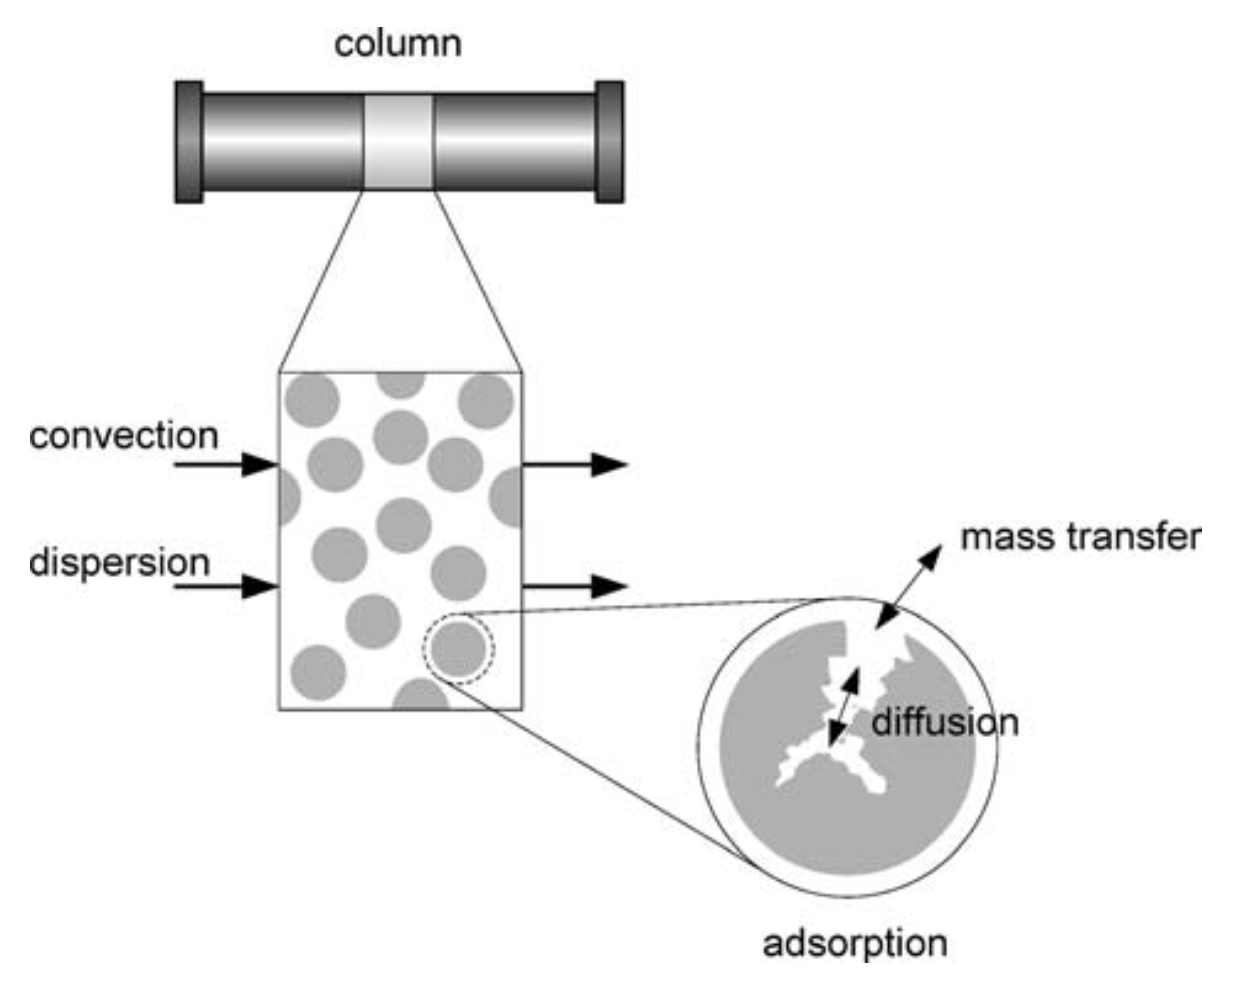
\includegraphics[width=0.55\textwidth]{diagramtransport.png}
\caption{Effects considered in chromatography model. Taken from Smith XX}
\end{figure}

\begin{itemize}
\item convection
\item Dispersion
\item Pore diffusion
\item Surface diffusion
\item adsorption kinetics
\item mass transfer from the mobile phase into the boundary layer of the stationary phase
\end{itemize}

In modeling liquid chromatographic processes, frequently different assumptions can be justified which lead to simplification in the mathematical models. The simplest model, known as the ideal model, neglects dispersion, pore and surface diffusion and mass transfer effects. On the other extreme, the most accurate model, known as the General Rate Model (GRM), consider all the phenomena listed above. In between, several models have been introduced in literature and are known as lumped transport models. Figure XX shows a simple diagram with the high-level classification of chromatography models and its corresponding variables.

Where $C$ represents the concentration in the mobile phase, $Cp$ the concentration in the pores of a bead, and $Q$ the concentration in the bead. For simplicity we describe here only the ideal model. Further details on more accurate models can be found in Guiochon et al. (2006) and Lieres and Andersson, 2010.

\begin{align}
& \frac{dc}{dt} = \left(\frac{1-\epsilon}{\epsilon}\right) \frac{dQ}{dt}-v\frac{dc}{dx} + D\frac{d^2C}{dx^2}\\
& a \frac{dQ}{dt} = f_{\text{ads}}(C,Q)
\end{align}

Given that the ideal model is the simplest model, and that it consist on a system of partial differential algebraic equations PDAEs, transport lumped models and the GRM are also system PDAEs, however, more complex and with a larger dimensionality. Despite its simplifications this ideal model is a good model to experiment and try ideas for the rigorous optimization.  
\\
\\
In pychrom the simulation of a chromatography columns can be done very efficiently with the GRM. A chromatography model is built in python and sent to the C++ software CADET, The Chromatography Analysis and Design Toolkit, to simulate the system. All the results are latter parsed and loaded into xarrays for easy post-processing in python
 

%%% End document
\end{document}